\section{پیش‌نمونه سازی
چیست}\label{ux67eux6ccux634ux646ux645ux648ux646ux647-ux633ux627ux632ux6cc-ux686ux6ccux633ux62a}

اکنون که شما بصورت اولیه میدانید که منظور من از آن \textbf{چیز}
\emph{درست} چیست، ما می‌توانیم مقدمه قابل قبول در باره پیش‌نمونه سازی
داشته باشیم. بهترین راه برای این کار بررسی دو داستانی است که من را به
فکر این موضوع انداخت: «آزمایش» تبدیل متن به گفتار آی بی ام و «آزمایش»
پالم پایلوت.

\section{آزمایش تبدیل گفتار به متن آی بی
ام}\label{ux622ux632ux645ux627ux6ccux634-ux62aux628ux62fux6ccux644-ux6afux641ux62aux627ux631-ux628ux647-ux645ux62aux646-ux622ux6cc-ux628ux6cc-ux627ux645}

اولین بار من این داستان را چند سال پیش در یک ارائه در یکی از کنفرانس‌های
نرم‌افزار شنیدم. من دقیقا نمی‌دانم تعاریف من از ماجراها چقدر دقیق است.
ممکن است من برخی از جزئیات را اشتباه دریافته باشم، اما نتیجه اخلاقی
ماجرا بسیار از جزئیات مهم‌تر است. با در نظر گرفتن این ایراد، این داستانی
است که من بخاطر می‌آورم.

چند دهه پیش، قبل از عصر اینترنت و حتی قبل از طلوع کامپیوترهای شخصی، آی
بی ام بخاطر ماشین تحریر و کامپیوترهای مینفریمش مشهور بود. در آن زمان
تایپ‌کردن یکی از ویژگی‌هایی بود که افراد کمی آنرا بخوبی انجام می‌دادند
که بیشتر آنها منشی، نویسنده و برخی از برنامه‌نویسان بودند. بیشتر افراد
از یک انگشت برا تایپ استفاده می‌کردند که کند و ناکارآمد بود.

آی بی ام درست در نقطه‌ای قرار داشت که بتواند از تجربه خود در بازار
کامپیوتر و ماشین تحریر استفاده کرده یک ماشین تبدیل متن به گفتار توسعه
دهد. این ابزار به افراد اجازه میداد که در یک میکروفن صحبت کنند و متن
بصورت «جادویی» روی صفحه نمایش ظاهر شود و دیگر نیازی به تایپ کردن نباشد.
این دستگاه پتانسیل زیادی برای کسب درآمد برای آی بی ام داشت و \emph{ریسک
بزرگ} روی این موضوع برای شرکت قابل قبول به نظر میرسید.

اما در این میان چندین اشکال بزرگ وجود داشت. کامپیوترها در آن زمان کم
قدرت تر و بسیار گرانتر از امروزه بوده و تبدیل متن به گفتار نیاز به
پردازش زیادی داشت. همچنین، با داشتن قدرت محاسباتی کافی، تبدیل متن به
گفتار یک مساله بسیار سخت علوم کامپیوتر بوده و هست. دست و پنچه نرم کردن
با این مساله نیاز به سرمایه‌گذاری عظیم -حتی برای آی بی ام- و سال‌های
زیاد برای تحقیق داشت. اما همه به این دستگاه نیاز داشتند. این یک موفقیت
واضح خواهد بود. یا اینطور خواهد شد؟

برخی در آی بی ام توسط افرادی که میگفتند به مردم تبدیل متن به گفتار «نیاز
داشته و قطعا آنرا خریداری نموده و استفاده میکنند» قانع نشده بودند و فکر
نمی‌کردند این دستگاه به موفقیت برسد. آنها از این می‌ترسیند که سال‌ها
تحقیق و سرمایه شرکت صرف توسعه دستگاهی شود که اندکی آنرا میخرند که این یک
فاجعه در کسب و کار است. به زبان پیش‌نمونه سازی آنها مطمئن نبودند که
تبدیل گفتار به متن یک \textbf{چیز} \emph{درست} است. همچنین، مردم تا کنون
از تبدیل گفتار به متن استفاده نکرده بودند ، پس آنها نمی‌توانستند بصورت
قطعی بدانند که کسی به این دستگاه نیاز دارد یا نه؟ آی بی ام نیاز به بررسی
قابلیت ماندگاری این دستگاه در کسب و کار را داشت اما ساختن حتی یک نمونه
اولیه نیاز به سال‌ها زمان داشت. آنها بجای آن یک آزمایش مبتکرانه طراحی
کردند.

آنها مشتریان بالقوه دستگاه تبدیل گفتار به متن خود را که به نظر آنها قطعا
خریدار این دستگاه بود در اتاقی با یک کامپیوتر، یک میکروفن و یک صفحه
نمایش بدون کیبرد قرار دادند. به آنها گفتند که یک ماشین تبدیل خودکار
گفتار به متن ساخته‌اند و میخواهند ارزیابی کنند که آیا مردم از استفاده از
آن لذت میبرند یا نه. وقتی آزمایش دهنده‌ها شروع به صحبت در میکروفن کردند
متن آنها تقریبا بی درنگ و بدون خطا روی صفحه نمایش ظاهر می‌شد! کاربران
تحت تاثیر قرار گرفته بودند. این برای واقعی بودن خیلی خوب بود که معلوم شد
نبوده است.

اتفاق پشت صحنه که این آزمایش را مبتکرانه میکند این بود که ماشین تبدیل
متن به گفتار حتی یک نمونه اولیه نبود. کامپیوتر موجود در اتاق خالی ساختگی
بود. در اتاق کناری یک تایپیست کارآزموده در حال گوش کردن به صدای کاربر
بود و با استفاده از کیبرد صحبت‌های او را تایپ و دستورات او را اجرا
میکرد. هرچه تایپیست تایپ میکرد روی صفحه نمایش کاربر نشان داده می‌شد.
صحنه سازی انجام شده به گونه‌ای بود که کاربر قانع میشد که خروجی روی صفحه
نمایش خروجی دستگاه تبدیل گفتار به متن است.

اما آی بی ام از این آزمایش چه یاد گرفت؟

این چیزی است که من شنیده‌ام: بعد از تاثیر اولیه بوسیله «تکنولوژی»،
بسیاری از افرادی که خریدار این سیستم بودند پس از چند ساعت کار با این
سیستم نظرشان عوض شد. گفتن چندین خط متن از طریق گفتار در کامپیوتر حتی با
استفاده تبدیل تقریبا بدون نقص و سریع توسط تایپیست هم دارای مشکلات زیادی
بود: گلوی افراد بر اثر صحبت زیاد خشک میشد، محیط کار پر از هم همه میشد و
به درد موارد محرمانه نمی‌خورد.

براساس نتایج این آزمایش، آی بی ام باز هم در تبدیل گفتار به متن سرمایه
گذاری نمود اما در مقیاسی به مراتب کمتر - آنها رو \emph{اعتبار شرکت قمار}
نکردند.

اینطور به نظر میرسد که این یک تصمیم درست در کسب و کار بوده است. کیبردها
نشان‌داده اند که در مورد وارد کردن متن به سختی شکست می‌خورند. سی سال پیش
مردم نمی‌توانستند تایپ کنند اما اکنون در هر دفتر (یا کافی شاپی) افراد
مختلف در سنین و شغل‌های مختلف را می‌بینید که در حال تایپ روی لپ‌تاپ‌های
خود هستند. در دستگاه‌هایی که کیبرد با سایز استاندارد غیر قابل استفاده
است همانند موبایل‌ها، تبدیل متن به گفتار میتواند یک \textbf{چیز}
\emph{درست} باشد اما در غیر اینصورت هنوز بایستی کیبرد را شکست بدیهد.
کیبرد قطعا یک \textbf{چیز} \emph{درست} است.

راهبرد آی بی ام مبتکرانه بود، اما شما به آن چه عنوانی می‌دهند. صحنه سازی
تبدیل گفتار به متن به کمک یک تایپیست قطعا یک «نمونه اولیه مناسب» نیست
مگر اینکه قصد داشته باشید که واقعا یک تایپیست زنده را درون یک کامپیوتر
جا بدهید. آنها یک نمونه اولیه از تبدیل متن به گفتار نساختند، بلکه
\emph{وانمود} کردند که یک نمونه اولیه تبدیل متن به گفتار داشته و از آن
به منظور دریافت عکس‌العمل مشتری به محصول استفاده کردند. در این حالت آنها
امکان جمع آوری اطلاعات با ارزش بازار را براساس استفاده واقعی به جای نظر
افراد داشتند، همچنین سرمایه‌گذاری مالی و زمانی کمی انجام دادند.

به نظر من این راهبرد بسیار ارزشمند و جالب است، و این روش به اندازه کافی
از ساختن نمونه اولیه متفاوت بوده که نام خاص خودش (که بیشتر در مورد آن
صحبت خواهم کرد) و ارزش بررسی را دارد. اما اول از هم سعی به یافتن
مثال‌های دیگر در این زمینه کردم که یک مثال عالی پیاده کردم.

\section{آزمایش پالم
پایلوت}\label{ux622ux632ux645ux627ux6ccux634-ux67eux627ux644ux645-ux67eux627ux6ccux644ux648ux62a}

آزمایش تبدیل گفتار به متن آی بی ام من را فکر در مورد مفهوم پیش‌نمونه
سازی واداشت، اما این مثال من را قانع کرد که این روش ارزش پیگیری را دارد

پالم پایلود در سال 1996 معرفی شد که به اندازه کف دست بوده و چهار عملیات
اصلی را انجام میداد: تقویم، دفتر تلفن، لیست کارهای روزمره و یادداشت
برداری ساده. پالم پایلوت اولین نمونه موفق دستیاران شخصی بود، اما جف
هاوکینز -یکی از بنیانگذاران پالم و کسی و مخترع پایلوت- به موفقیت
دستیارهای شخصی مطمئن نبود. برعکس باتوجه به مقاله سال 1998 در مجله
تایمز(تاکیدها را من اضافه کرده ام):

\begin{quote}
هاوکینگ ۴۰ ساله، مدیر تکنولوژی پالم و مخترع پالم، یکی از اولین
کامپیوترهای قابل حمل به نام گریدپد را ده سال پیش ساخته است. این کامپیوتر
یک \textbf{پدیده اعجاز انگیز مهندسی اما یک شکست تجاری} بود به خاطر اینکه
به نظر او هنوز بسیار بزرگ بود. وقتی همکاران او از او پرسیدند که
کامپیوترهای جدید چه اندازه ای باید باشد \textbf{برای اطمینان از اینکه
این اشتباه را دوباره تکرار نکند} برای آنها جواب آماده‌ای داشت: «بیایید
سایز لباس را \textbf{آزمایش کنیم}»
\end{quote}

\begin{quote}
او به گاراژ خود بازگشت و یک تکه چوب را به اندازه سایز جیب لباس خود برید.
سپس او این تکه چوب را در ماه‌های متمادی حمل کرد و با \textbf{تظاهر} به
اینکه آن تکه چوب واقعا یک کامپیوتر است. آیا او برای ناهار چهار شنبه آزاد
بود؟ هاوکینز آن تکه چوب را از جیبش خارج میکرد و انگار که دارد برنامه
زمانی خود را چک میکند آنرا میفشرد. اگر او به شماره تلفنی نیاز داشت، او
\textbf{تظاهر} به پیدا کردن آنرا در قطعه چوب میکرد. معمولا او طراحی
ظاهری متفاوتی را با چینش دکمه‌های متفاوت رو کاغذ پرینت میکرد و با
چسباندن آنها روی چوب طراحی جدید را امتحان میکرد.
\end{quote}

این عکس پیش‌نمونه‌ای است که جف آنرا ساخته است(شما میتوانید نمونه‌های
بیشتری در موزه تاریخچه کامپیوتر در مانیتن ویوو کالیفرنیا پیدا کنید).

\begin{figure}[htbp]
\centering
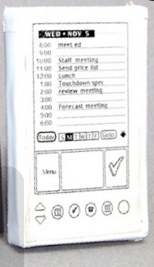
\includegraphics{palmpilot.png}
\caption{پیش نمونه پالم پایلود}
\end{figure}

من فقط میتوانم عکس العمل دیگران را هنگامی که هاوکینز آن تکه چوب را از
جیب خود بیرون می‌آورد و آنرا همانند یک کامپیوتر فعال میفشرد تصور کنم.
آنها فکر میکردند که او دیوانه شده است. اما نه او بسیار باهوش بود. آن تکه
چوب به همراه دکمه‌های پرینت‌شده هاوکینز را به این نتیجه رساند که او راه
درستی را آمده است. او برای اولین و مهمترین سوال پاسخی یافته بود: «اگه من
یک پایلوت داشتم، آیا آنرا با خود حمل کرده و از \textbf{آن چیز} استفاده
میکردم؟» و جواب قطعا «بله» بود و او میدانست که \textbf{چیز} \emph{درست}
را یافته است. اکنون او می‌توانست روی سوالات بعدی تمرکز کند مانند: آیا
می‌توانم آنرا کوچک درست کنیم؟ ساخت آن چقدر هزینه خواهد برد؟ عمر باتری‌ها
چقدر خواهد بود؟ اکنون زمان ساخت یک «نمونه اولیه مناسب» رسیده بود.

پالم پایلوت تنها موفق نبود بکله یک موفقیت بسیار بزرگ با تاثیر عظیم بود.
پایلوت جد تمامی تلفن‌های هوشمند امروزی است. این محصول تنها از تکه چوبی
شروع شد همانند پینوکیو.

\section{وانمود کنید قبل از اینکه
بسازید}\label{ux648ux627ux646ux645ux648ux62f-ux6a9ux646ux6ccux62f-ux642ux628ux644-ux627ux632-ux627ux6ccux646ux6a9ux647-ux628ux633ux627ux632ux6ccux62f}

داستان‌های تبدیل متن به گفتار و پالم پایلوت چیزهای مشترک بسیاری دراند.

\begin{quote}
هر دو تیم شک‌های زیادی درباره سودمندی و قابلیت استفاده و پذیرش ایده خود
داشتند. هر دو ایده جالب بود. درست به نظر میرسیدند. مساله‌ای را حل
می‌کردند. اما آیا آنها یک \textbf{چیز} \emph{درست} بودند؟ آیا مردم واقعا
از آنها استفاده می‌کردند؟ جف هاوکینز حتی سالهای زیادی را برای توسعه
محصول (گریدپد) که «پدیده اعجاز انگیز مهندسی اما یک شکست تجاری بود»، از
دست داده بود(یک \textbf{چیز} \emph{غلط}) و تصمیم داشت که «این اشتباه را
دوباره تکرار نکند».
\end{quote}

\begin{quote}
بخاطر شکشان هر دو تیم میخواستند کاربردپذیری و سودمندی ایده‌هایشان را با
ساختن یک نمونه اولیه آزمایش کنند. همچنین قبل از اینکه شروع به توسعه
محصول کنند، بازخوردهای \emph{استفاده واقعی از محصول}(بجای \emph{نظرات در
مورد محصول}) را جمع آوری کنند.
\end{quote}

\begin{quote}
در هر دو آزمایش اما توسعه حتی یک «نمونه اولیه مناسب»(نسخه خام ولی
عملیاتی محصول نهایی) زمان بسیار و سرمایه‌گذاری قابل توجهی برای تحقیق و
توسعه نیاز داشت.
\end{quote}

\begin{quote}
راه حل آنها برای مشکل «نمونه اولیه مناسب» این بود که \emph{تظاهر} به
داشتن یک چنین نمونه اولیه‌ای کنند. در مثال تبدیل گفتار به متن، سخت افزار
و نرم‌افزار با کمی حیله گری جایگزین شده بود و در پالم پایلوت با قوه تخیل
هاوکینز جایگزین شده بود. \emph{وانمود کنید قبل از اینکه آنرا بسازید}
\end{quote}

به نظر من این دو داستان بخاطر تفاوت بسیار از آنچه افراد و کمپانی‌ها
بصورت معمول در پیگیری ایده‌های نوشان انجام می‌دهند قابل توجه و موثر
بودند. بیشتر مردم عاشق ایده‌ی شان می‌شوند(آن \textbf{چیز} آنها) و فرض
می‌کنند که آن \textbf{چیز} موفق خواهد بود(آن \textbf{چیز} \emph{درست})
پس شروع به ساختن آن می‌کنند. آنها پیش از موعد شروع به تمرکز و
سرمایه‌گذاری روی چیزهای غلط در زمان غلط می‌کنند. بصورت دقیق‌تر، آنها
بیشتر از نیاز و پیش از موعد روی توسعه اولین نسخه محصول خود که دارای
ویژگی‌های زیاد، کارکردهای بیش از حد و «رنگ و لعاب» بیش از حد نیاز است،
سرمایه‌گذاری می‌کنند. آنها پیش‌فرضشان بر این است که مردم آنرا خواهند
خواست. در بسیاری از موارد، این پیش‌فرض ها و فرضیات هم غلط و هم پر هزینه
از کار در می آیند.
